\documentclass[10pt,a4paper,twocolumn,twoside,UTF8]{ctexart}
\usepackage{geometry}
	\geometry{left=2cm,right=2cm,top=2.5cm,bottom=3cm}
\usepackage{xeCJK,amsmath,paralist,enumerate,booktabs,multirow,graphicx,subfig,setspace,listings}
	\setlength{\parindent}{2em}%正文首行缩进两个汉字
	\lstset{language=tex}
\usepackage{titlesec}
	\newfontfamily\sectionef{Times New Roman}
	\setCJKfamilyfont{FZHeiTi}{黑体}
	\newcommand{\sectioncf}{\CJKfamily{FZHeiTi}}
	\titleformat*{\section}{\large\bfseries\sectioncf\sectionef}
	\titleformat*{\subsection}{\normalsize\bfseries\sectioncf\sectionef}
\usepackage{fancyhdr}
\usepackage{layout}
\setlength\columnsep{0.8cm}%设置双栏的间距


%%begin----------设置首页和正文不同的页眉页脚----------------%%

\usepackage{ifthen}%这个宏包提供逻辑判断命令
\newboolean{first}%引入布尔变量
\setboolean{first}{true}%将布尔变量设置为true
\pagestyle{fancy}

	\fancypagestyle{maincontent}{
		\fancyhf{}  %清空页眉页脚设置
		\fancyhead[EL, OR]{\thepage}
		\fancyhead[EC]{实验B2 不良导体热传导率的测量(准稳态法)}
		\fancyhead[OC]{基\quad 础\quad 物\quad 理\quad 实\quad 验}
		\renewcommand\headrulewidth{0pt}
	}

	%%% Step2 定义首页的页面风格
	%页眉中间的双行文字,大小和字间距需要微调
	%左右的内容是年月,可以自己修改寻找自动获取的方法
	\usepackage{datetime}
		%\shortmonthname可以获取英文月份缩写
	\fancypagestyle{firstpage}{
		\setboolean{first}{false}%firstpage出现,则将first重置为false
		\fancyhf{}  %清空页眉页脚设置
		\fancyhead[L]{\the\year 年\the\month 月}
		\fancyhead[R]{\shortmonthname[\the\month], \the\year}
		\fancyhead[C]{
		\large{基\quad 础\quad 物\quad 理\quad 实\quad 验}\\
		\normalsize{GENERAL PHYSICS LABORATORY}
		}
	}

	%%% Step3 页眉线的设置:用布尔变量区分首页和正文
	\newcommand{\makefirstpageheadrule}{%定义首页页眉线-双线绘制命令
	\makebox[0pt][s]{\rule[0.6\baselineskip]{\headwidth}{0.3pt}}
	\makebox[0pt][s]{\protect\hspace{-0.34em}\rule[0.75\baselineskip]{\headwidth}{0.3pt}}
	\protect\vspace{-20pt}
	%\rule[9pt]{\headwidth}{0.3pt}
	% \rule[25pt]{\headwidth}{0.3pt}
	%\rule[raise-height]{width}{height}
	%其中第一个可选参数为将直线抬多高
	}

	\newcommand{\makeheadrule}{%定义正文页页眉线绘制命令,单线
	\makebox[0pt][l]{\rule[1\baselineskip]{\headwidth}{0.3pt}}
	\protect\vspace{-20pt}%页眉和正文的距离
	}

	%根据布尔变量first为true或false分别执行不同的页眉线绘制命令
	\renewcommand{\headrule}{%重定义headrule命令
	\ifthenelse{\boolean{first}}{\makeheadrule}
	{\makefirstpageheadrule}
	}


%%end--------------设置首页和正文不同的页眉页脚-----------%%



%%begin-----------------参考文献-----------------------%%

\usepackage[colorlinks,linkcolor=blue,urlcolor=blue]{hyperref}%超链接
\usepackage[hyperref=true,backend=biber,bibstyle=gb7714-2015,citestyle=numeric-comp,sorting=none,backref=true]{biblatex}
	%hyperref=true和backref=true表示为各个参考文献的引用处、及定理、定义、例子等的引用处都添加上超链接;
	%backend=biber:后端处理的程序为biber.exe
	%bibstyle:参考文献风格;每个期刊、组织要求不同
		%gb7714-2015是目前国内期刊通用的风格,称为gb标准风格
	%citestyle:引用风格;每个期刊、组织要求不同
	%sorting=none:按照参考文献在论文中出现的先后顺序排序。
	%**编译:biblatex与biber命令配合使用。xelatex-biber-xelatex-xelatex
\addbibresource{book.bib}
	%这里写上.bib文件的相对地址
	%每次实验引用的页数不同,需要手动改变

%%end-------------------参考文献-----------------------%%





%%%%%%%%%%%%%%%%%%%%%%%%%%%%%%%%%%%%%%%%%%%%%%%%%%%%%%%%%%
%%%%%%%%%%%%%%%%%%%%%%%%%正文开始%%%%%%%%%%%%%%%%%%%%%%%%%%
%%%%%%%%%%%%%%%%%%%%%%%%%%%%%%%%%%%%%%%%%%%%%%%%%%%%%%%%%%

\begin{document}


%%begin-------------------中文摘要-----------------------%%
\title{\LARGE\textbf{不良导体热传导率的测量(准稳态法)}\footnotemark[1]}
\author{\large\textit{XXX xxxxxxxx}$^{1}$\footnotemark[2]
\\ \normalsize{(1 \textit{中山大学 物理学院,广东 广州 }510275)}}
\date{}%不显示日期

\twocolumn[
	\begin{@twocolumnfalse}
	\maketitle  
  	\renewcommand{\abstractname} {} 
	\begin{abstract}
	\vspace{-3em}
	{\bf 摘{} 要:}
	{\small 热导体导热遵循热传导方程。
    导热系数和比热是描述热导体导热性能的两个重要参量。
    本实验中,我们基于热电偶测温,采用准稳态法测量有机玻璃材料和橡胶材料的导热系数与比热,以探究不良导体的导热规律。
    实验测得有机玻璃材料比热为$2105.82 J kg^{-1}\ ^{\circ}C^{-1}$,导热系数为$\lambda = 0.264 Wm^{-1}K^{-1}$;
    橡胶材料比热为$1771.38 J kg^{-1}\ ^{\circ}C^{-1}$,导热系数为$\lambda = 0.658 Wm^{-1}K^{-1}$。}
	\par
	\textbf{关键词}:准稳态法,不良导体,热电偶,比热,导热系数
	\vspace{2em}
	\end{abstract}
	\end{@twocolumnfalse}
]
\renewcommand{\thefootnote}{\fnsymbol{footnote}}
\footnotetext[1]{由中山大学物理学院陆佑堂提供器材和指导。}
\footnotetext[2]{通信作者,\url{xxxx@mail2.sysu.edu.cn}}
%%end-------------------中文摘要-----------------------%%


\thispagestyle{firstpage}%首页页面风格:firstpage
\pagestyle{maincontent}%第二页之后的页面风格:maincontent


%%begin----------------层级结构------------------------%%

%重点1:知道每一个层级的样式和怎么和后面的正文接上
%重点2:掌握各种换段的方法
%重点3:自定义的项目符号(宏包enumerate的用法)

\section{引 \quad 言}
热传导是热传递三种基本方式之一。
导热系数定义为单位温度梯度下每单位时间内由单位面积传递的热量,单位为 $W/( m \cdot  K )$。
它表征物体导热能力的大小。

比热是单位质量物质的热容量。
单位质量的某种物质,在温度升高(或降低)1度时所吸收(或放出)的热量,叫做这种物质的比热,单位为 $J /( kg \cdot K )$。

测量导热系数和比热通常都用稳态法,使用稳态法要求温度和热流量均要稳定,但在实际操作中要实现这样的条件比较困难,因而会导致测量的重复性、稳定性、一致性较差,误差也较大。

为了克服稳态法测量的这些弊端,本实验使用了一种新的测量方法——准稳态法,使用准稳态法只要求温差恒定和温升速率恒定,而不必通过长时间的加热达到稳态,就可以通过简单的计算得到导热系数和比热。
\newpage
%换一栏,而不是换一页。换一页用\clearpage

\section{介\quad 绍}
%在论文写作中, 我们通常用到的\LaTeX 中的层级结构如下, 包括会进入pdf目录的章节结构\lstinline|\section|, \lstinline|\subsection|, \lstinline|\subsubsection|和不会进入目录的段落结构\lstinline|\paragraph|, \lstinline|\subparagraph|.
    \subsection{准稳态法测量原理}
	\begin{figure}[!h]
		\centering
		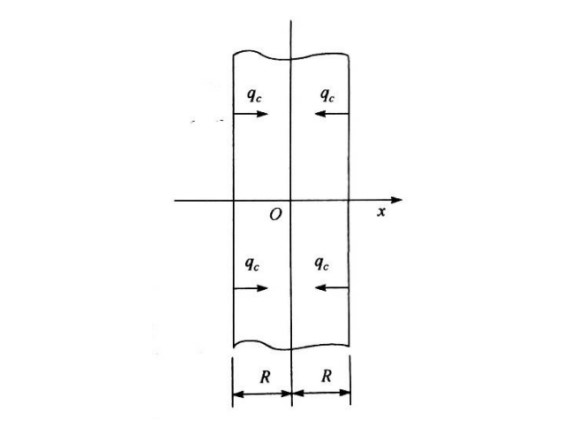
\includegraphics[width=0.4\textwidth]{img//1.jpg}
			%textwidth:正文宽度。双栏,则将两栏正文宽度相加。
		\caption{理想无限大不良导体平板}
		\label{fig:1}
	\end{figure}

	考虑如图\ref*{fig:1}所示的一维无限大导热模型,一无限大不良导体平板厚度为2R,初始温度为$t_0$,在平板两侧同时施加均匀的指向中心面的热流密度$q_c$,则平板上各处的温度将随加热时间$\tau$ 而变化,故x处的温度可表示为 $t ( x , \tau )$.如\ref*{fig:1}所示,以样品中心为坐标原点,则上述模型的热运动方程可写为: 
	\[\left\{%\left和\right配合使用,可以得到大小匹配的各种括号
	\begin{aligned}
	&\partial t ( x , \tau )/\partial \tau=a\partial ^2 t ( x , \tau )/\partial x^2\\
	&\partial t ( R , \tau )/\partial x=q_c/\lambda, \partial t ( 0 , \tau )/\partial x =0\\
	&t(x,0)=t_0
	\end{aligned}
	\right.
	\]
	
    其中,$a=\lambda/\rho c$;$q_c=c \rho R\partial t/\partial \tau$;
	$\lambda$为材料的导热系数;$\rho$ 为材料密度;c为材料的比热。当加热时间$\tau$ 满足$a\tau/R^2>0.5$时,$\tau$ 的求和项可忽略,方程的解为:
	\begin{equation*}
		t(x,\tau)=t_0+\frac{q_c}{\lambda}\left(\frac{a}{R}\tau+\frac{1}{2R}x^2-\frac{R}{6}\right)
	\end{equation*}

	被测样品中心和表面处的温度分别为:
	\[\left\{%\left和\right配合使用,可以得到大小匹配的各种括号
	\begin{aligned}
	&t(0,\tau)=t_0+\frac{q_c}{\lambda}\left(\frac{a}{R}\tau-\frac{R}{6}\right)\\
	&t(R,\tau)=t_0+\frac{q_c}{\lambda}\left(\frac{a}{R}\tau+\frac{R}{3}\right)\\
	\end{aligned}
	\right.
	\]

	两处的温度随加热时间线性上升,升温速率为 $a q_c / \lambda R$ ,这是一个与材料导热性能和实验条件有关的参数。
	而加热面和中心面间的温度差为:
	\begin{equation*}
		\varDelta t=t(R,\tau)-t(0,\tau)=q_c R/2 \lambda
	\end{equation*}
	可见,该状态下被测样品各处匀速升温,而$\varDelta t$与加热时间$\tau$无关并保持恒定,这种状态称讨论为准稳态。
	则样品的导热系数为
	\begin{equation*}
		\lambda=q_c R/2\varDelta t
	\end{equation*}
	样品的比热为:
	\begin{equation*}
		c=q_c/(\rho R dt/d\tau)
	\end{equation*}
    其中,$dt/d\tau$ 为样品的升温速率,准稳态,样品各处的升温速率相等。可见,只要测出准加热稳态下样品表面和中心处的温度差及样品的升温速率,就可以计算出被测样品的热导率$\lambda$和比热 c .

	\section{实验仪器和样品}
    \subsection{比热/导热系数实验仪(ZKY-BRDR)}
	比热/导热系数实验仪具备为加热器提供电源、测量加热时间以及测量热电偶热电动势的功能,可以方便测量导体比热/导热系数。
	实验仪面板如图\ref{fig:illus-2}所示。
	\begin{figure}[!h]
        \centering
        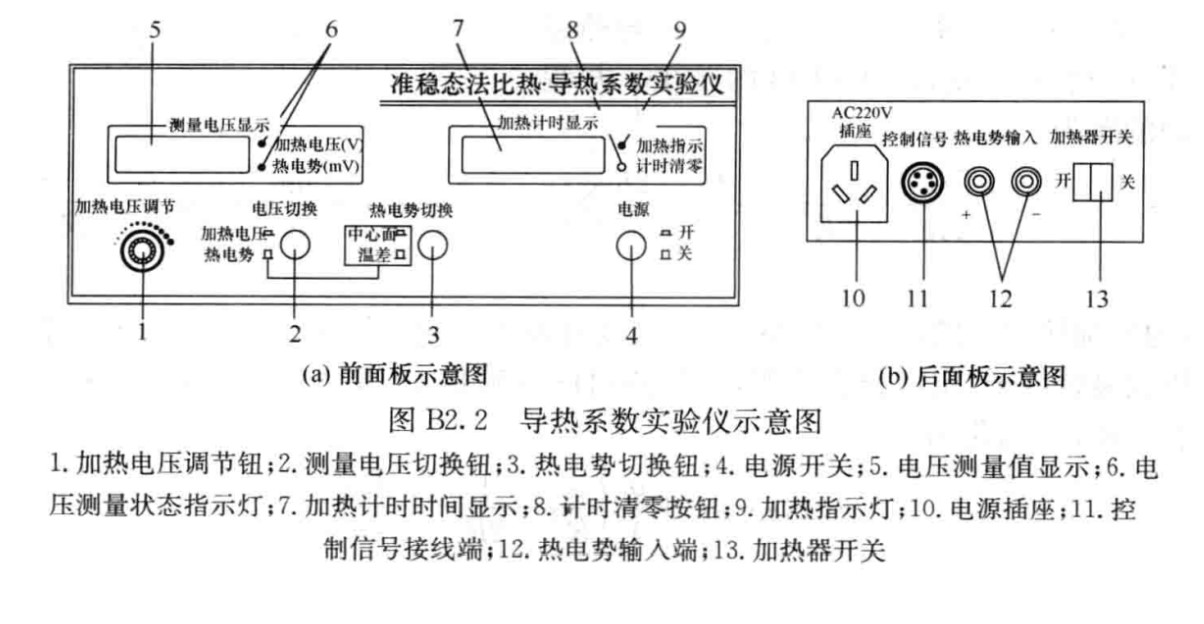
\includegraphics[width=0.4\textwidth]{img//2.jpg}
        \caption{比热/导热系数实验仪}
        \label{fig:illus-2}
    \end{figure}
	
	需注意的是实验仪只有一个电压输入端口,因此需使用测控电路切换待测电压。

	\subsection{带保温杯的样品架}
	样品架与保温杯如图\ref{fig:illus-3.1}所示。热电偶接线如图\ref{fig:illus-3.2}所示

	\begin{figure}[!h]
        \centering
        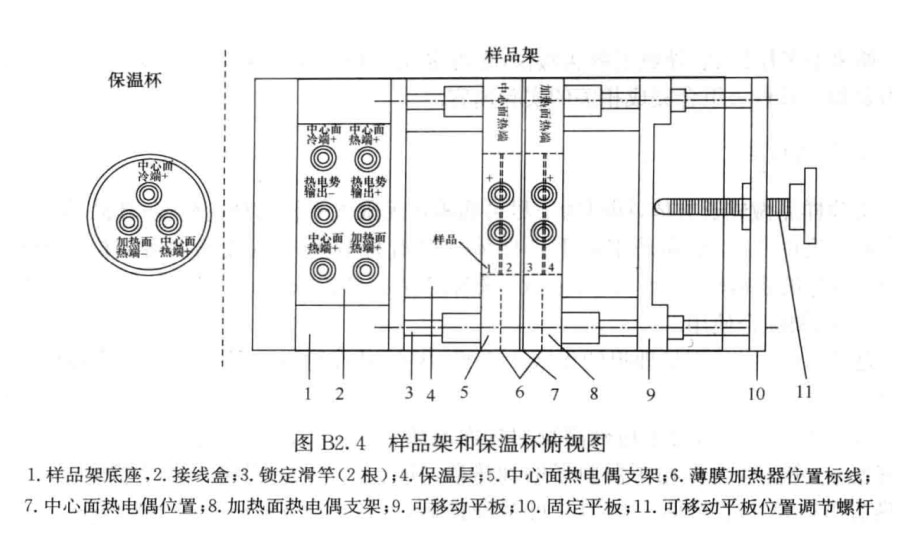
\includegraphics[width=0.4\textwidth]{img//3.jpg}
        \caption{样品和保温杯俯视图}
        \label{fig:illus-3.1}
    \end{figure}
	\begin{figure}[!h]
        \centering
        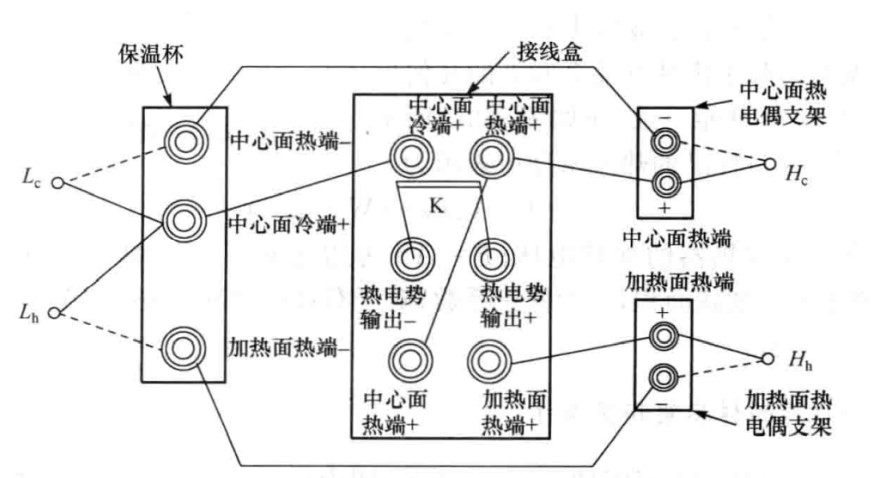
\includegraphics[width=0.4\textwidth]{img//4.jpg}
        \caption{比热/导热系数实验线路连接示意图}
        \label{fig:illus-3.2}
    \end{figure}

		\subparagraph*{保温杯} 可以提供恒温冷端。实验中将两热电偶冷端接触后放入保温杯中,以保证两热电偶冷端温度相同。
		\subparagraph*{调节螺钉} 旋动螺钉,可以夹紧或松开样品架,以取放样本。
		\subparagraph*{铜-铜镍热电偶} 将温度信号转换为热电势信号,测量温度。
		\subparagraph*{接线盒} 放大热电势信号,以减少信号干扰;内置继电器,可以切换输出中心面热电势$U_C$和温差热电势$\Delta U$。
	
    \subsection{待测样品与装置}
	本实验测量样品为有机玻璃(密度$\rho = 1196 kg/m^3$)与橡胶(密度$\rho = 1374 kg/m^3$)。

	为尽可能贴近无限大导热模型,样品形状为正方形薄板。然而,样品并非理想无限大导热模型,因此在计算面积时应引入边缘修正。修正后加热面积$F$为
	\begin{equation}
		F = \frac{S}{A}
	\end{equation}
	$S$为实际面积,$A$为修正系数,取为$A=0.85$。

	样品在样品架中的装置如图\ref{fig:illus-4}。
	\begin{figure}[!h]
        \centering
        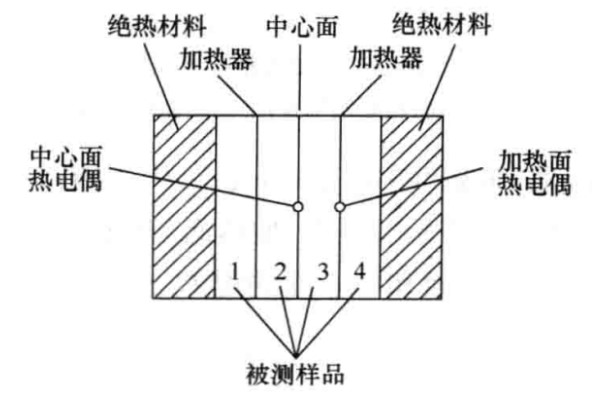
\includegraphics[width=0.4\textwidth]{img//5.jpg}
        \caption{样品在样品架中的装置}
        \label{fig:illus-4}
    \end{figure}
	四块样品两两夹持薄膜加热器,保证样品均匀加热且两侧热阻相同,则热流密度$q_c$为加热功率的一半。
	\begin{equation}
		q_c = \frac{U^2}{2Fr}
	\end{equation}
	$U$为加热电压,$r$为加热器电阻。
	
	两测温热电偶分别在中心面和其中一个加热面。


	\section{实验步骤}
	\subsection{测量有机玻璃样品的导热系数和比热容}
	\begin{enumerate}
		\item 测量样品儿何尺寸、共有四个样品
		\item 安装样品并连接线路、旋松螺杆旋钮,轻轻拔出中心面热电偶支架和加热面热电凰支架,露出样品架。
		戴好手套,将冷却好的“有机玻璃”样品放人样品架,样品2和3采用厘度最接近的两个样品,然后旋转螺杆旋钮压紧样品
		\item 设定加热电压,确认实验仪后面板上的“加热控制”开关已经关闭,再打开主机电源,预热约10min。将“电压切换”按钮切换至“加热电压”挡,旋转“加热电压调节”旋钮到所需要的电压(参考加热电压:17-19V)
		\item 测定样品“加热面与中心面”间的温度差和“中心面”的升温速率,将“电压切换”按钮切换至“热电势”挡,将“热电势切换”按钮切换至“温差”挡、耐心等待,直至“温差执电势”显示值小于0.04mV(约$1^{\circ }C$)。打开测试仪后面板的“加热控制”开关开始升温,每隔30s或1min记录一次“加热面与中心面温差热电势”和“中心面热电势”由于测试仪加热功率有限,中心面温度过高时,升温谏率会降低而偏离线性,所以每次升温时间应控制在15min左右,最长不大于25min。
		\item 计算“加热面与中心面温差”及“中心面温度”,并作出它们随时间的变化关系曲线。在准稳态状态下,选取合适的数据计算机玻璃的导热系数入和比热容 c ,准稳态需同时满足 $a\lambda / R >0.5$和“中心面温度”线性上升两个条件
	\end{enumerate}

	\subsection{测量橡胶样品的导热系数和比热容}
	采用橡胶样品,按上述方法完成实验,并作图。计算出橡胶的导热系数$\lambda$和比热容c.


\section{数据处理与分析}
实验参数:

加热电压:$U=18V$

有机玻璃、橡胶密度分别为:

$\rho_{1} = 1196 kg/m^3$,$\rho_{2} = 1374 kg/m^3$

修正后加热面积:

$F=S/A=0.09m\times0.09m/0.85=9.529m^2$

有机玻璃、橡胶样品平均厚度:

$R_1=10.0555mm$,$R_2=10.1795mm$

铜-铜镍热电偶电压温度系数为$0.04mV/^{\circ}C$

总内阻$r=110\varOmega$

室温$22^{\circ}C$

通过样品的热流密度:$q_c = \frac{U^2}{2Fr}=214W/m^2$

\subsection{测有机玻璃样品的导热系数和比热容}
\begin{figure}[!h]
	\centering
	\subfloat[]{\label{fig:6a}
	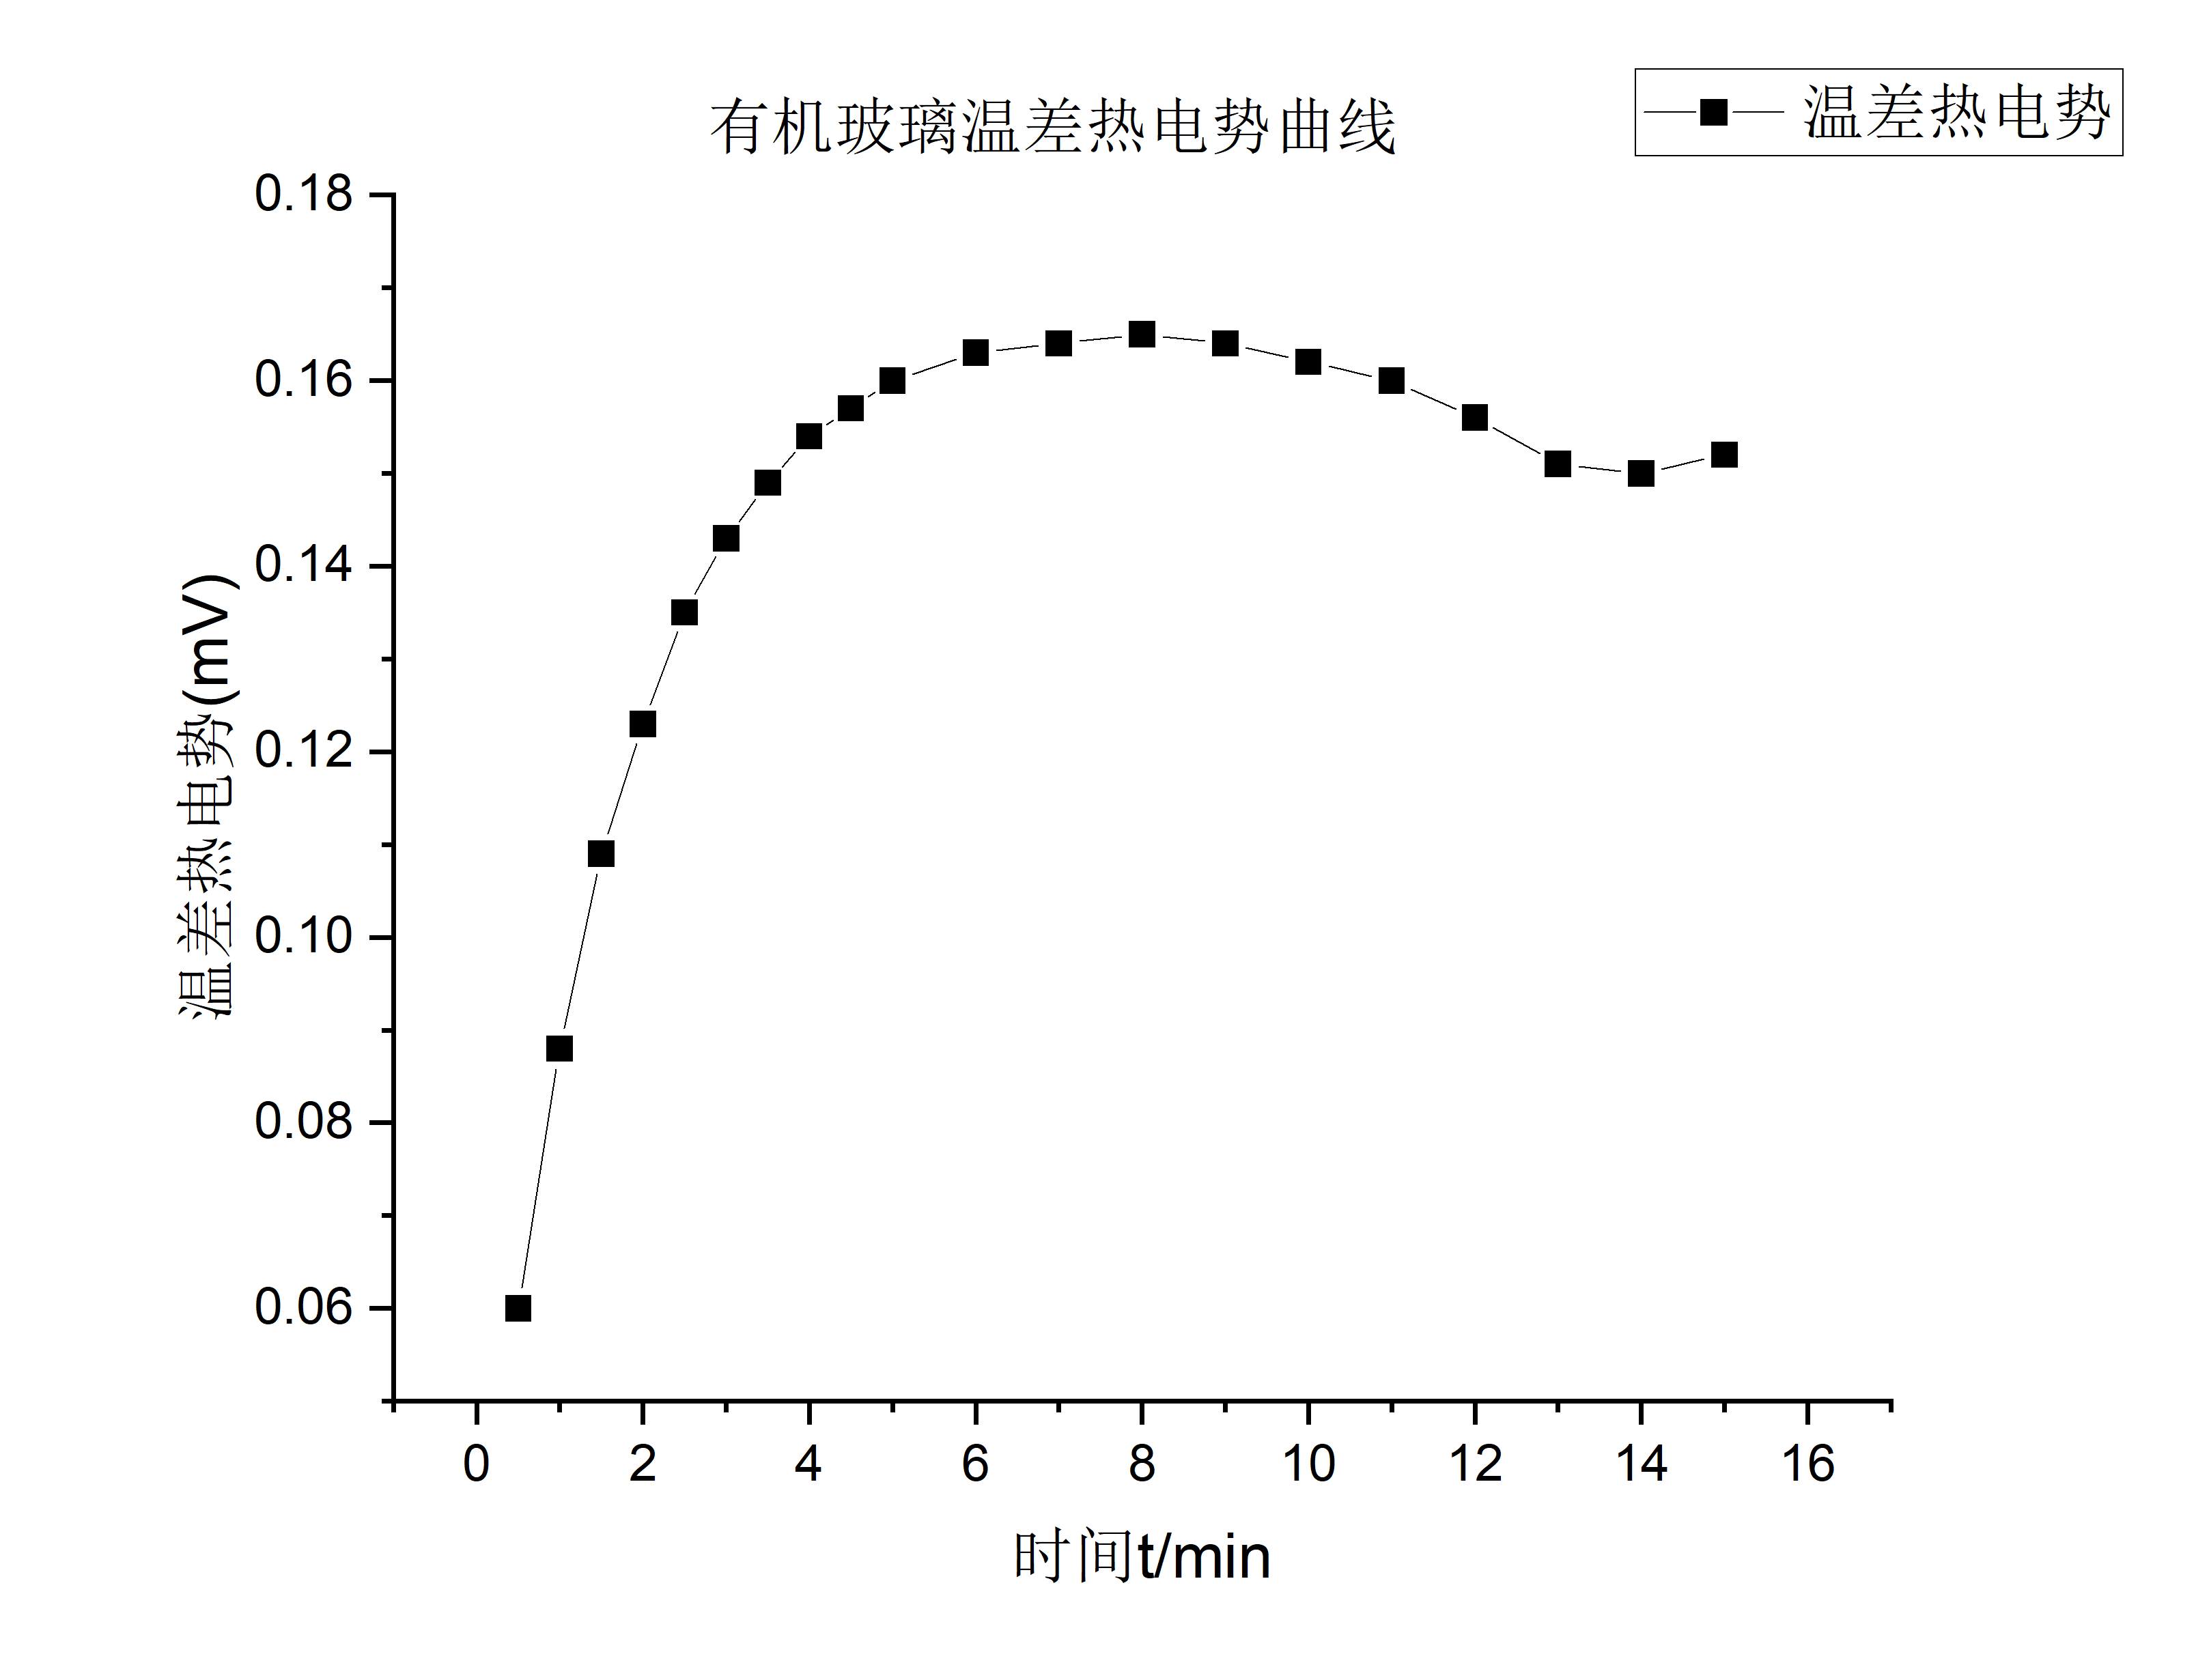
\includegraphics[width=0.23\textwidth]{img//6a.png}
	}	
	\subfloat[]{\label{fig:6b}
	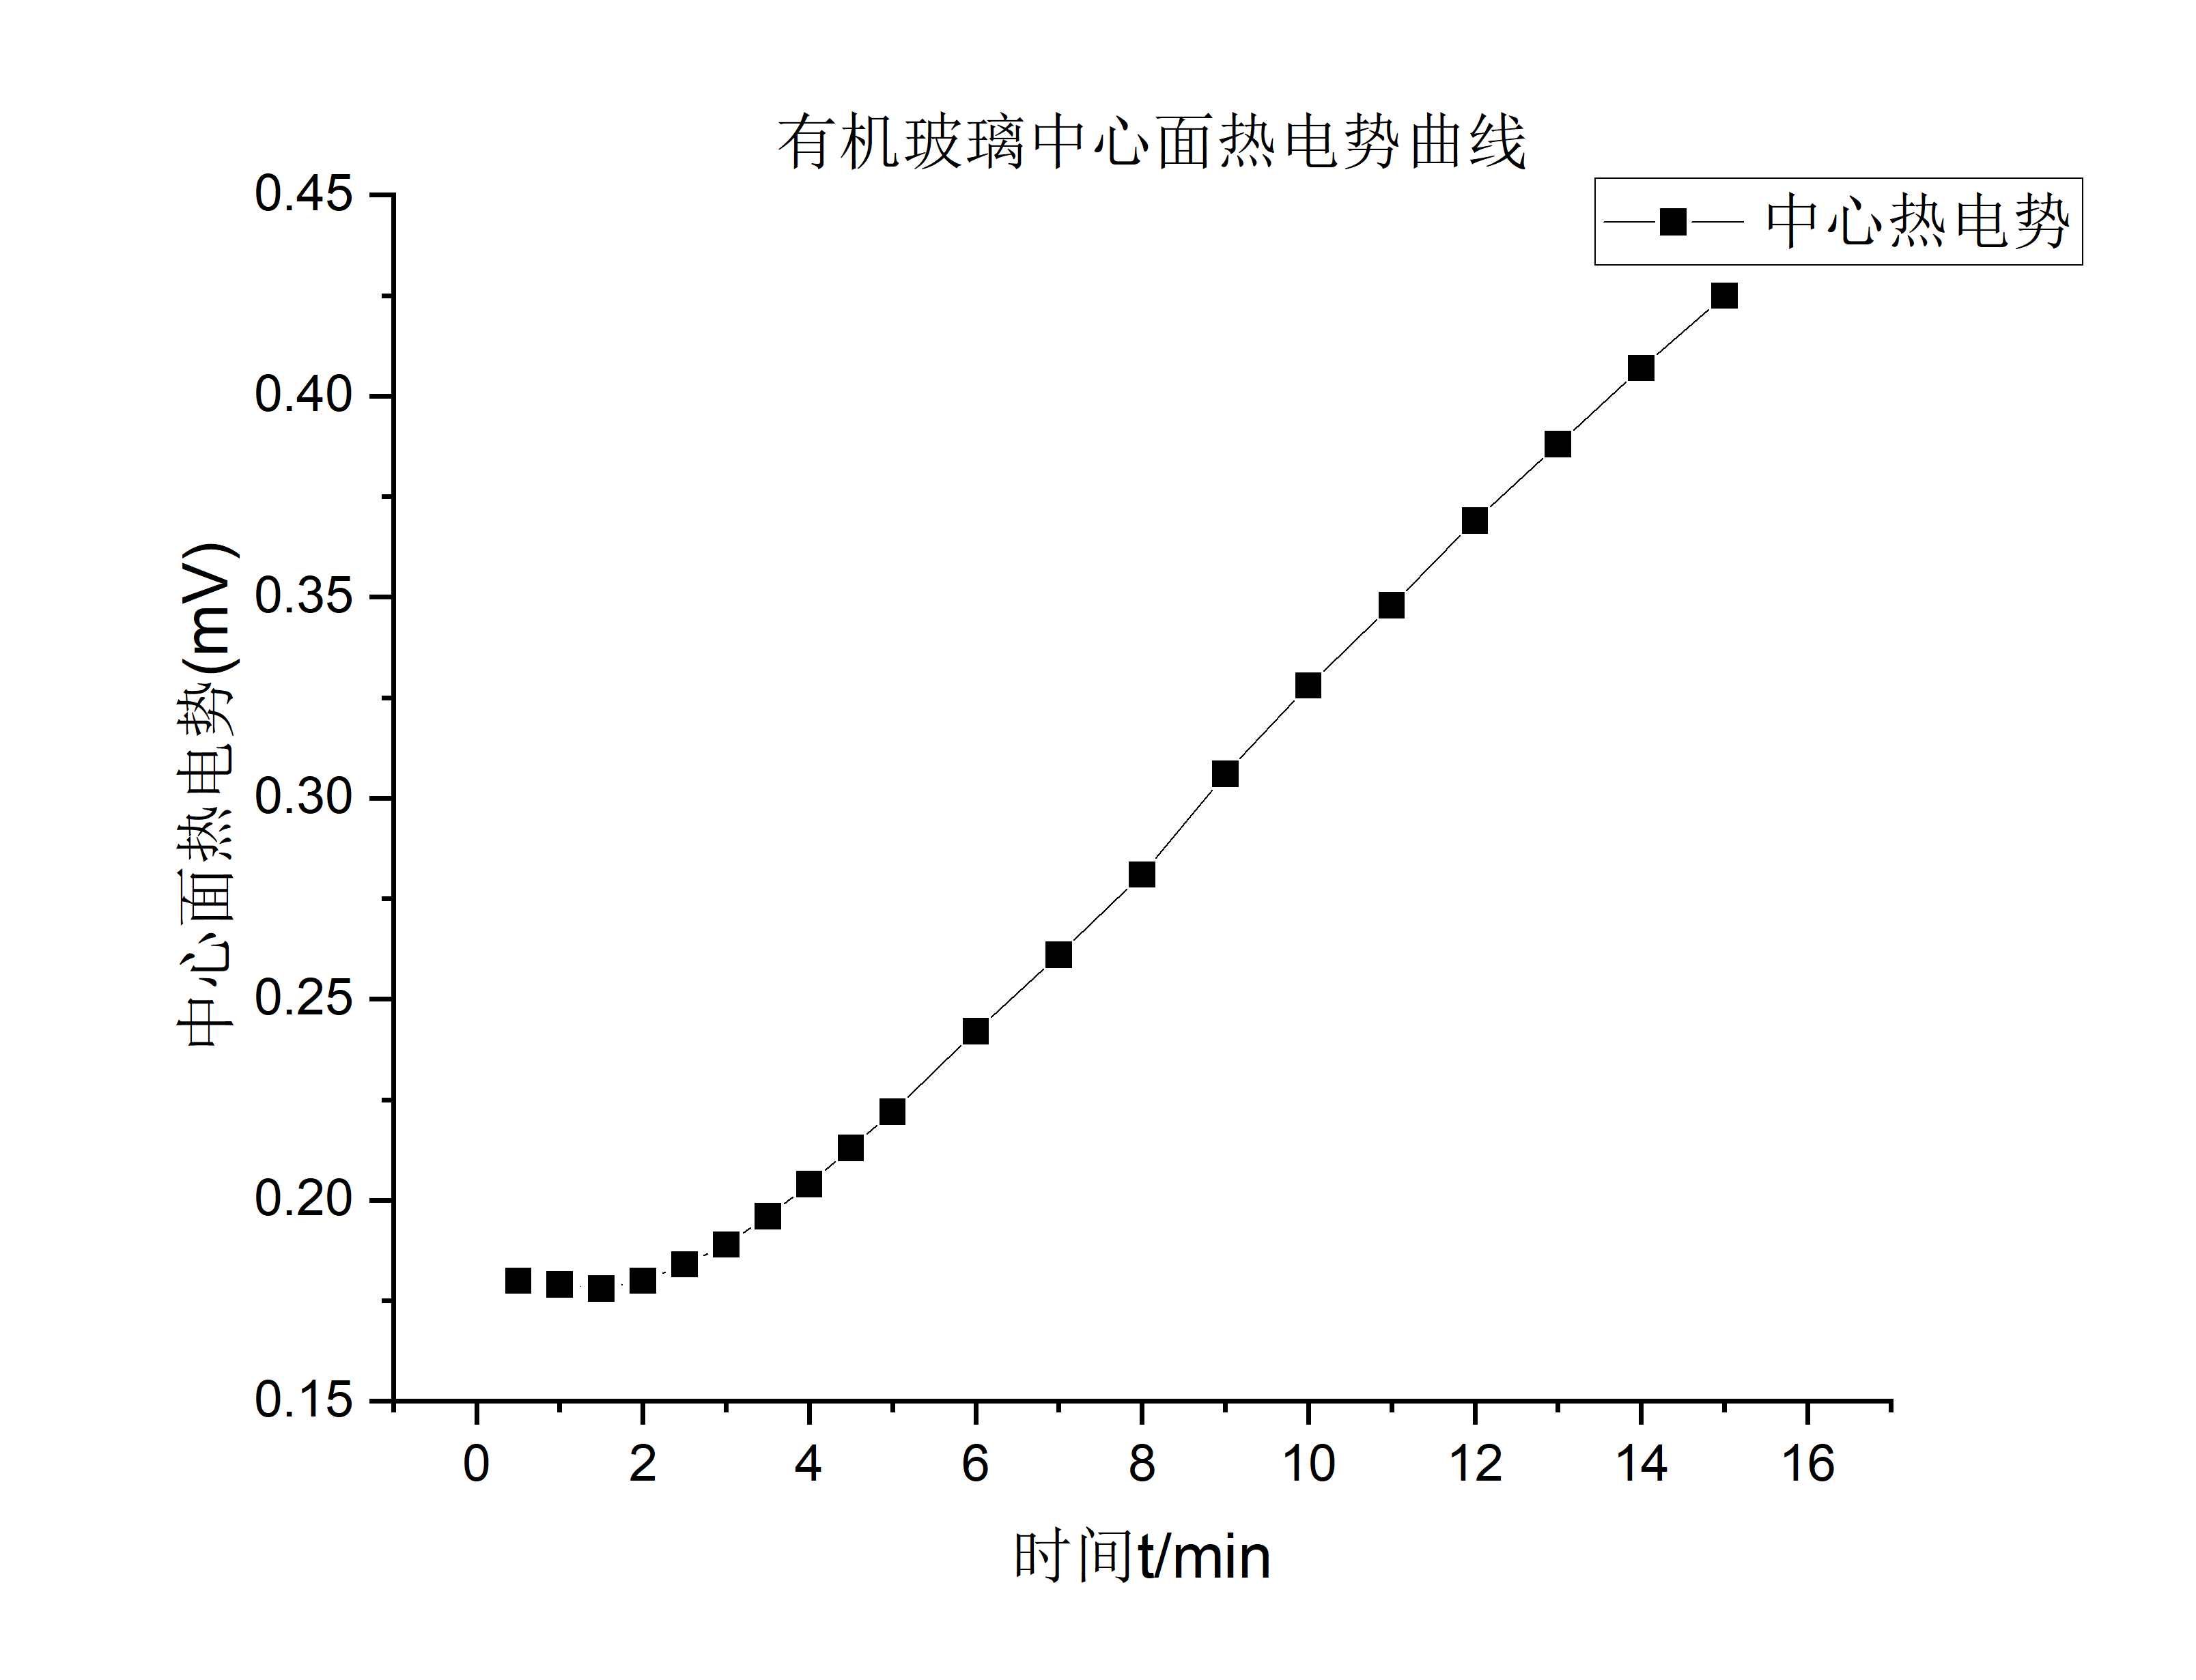
\includegraphics[width=0.23\textwidth]{img//6b.png}
	}
	\caption{有机玻璃实验数据}
\end{figure}

由实验记录得,在第6分钟处于准稳态。此时温差热电势$V_t=0.163mV$.

\begin{align*}
	&\varDelta t =\frac{V_t}{0.04}=4.075K\\
    &\lambda=\frac{q_c R_1}{2\varDelta t}=0.264W/mK
\end{align*}

计算得热导系数$\lambda=0.264mK$

\begin{figure}[!h]
	\centering
	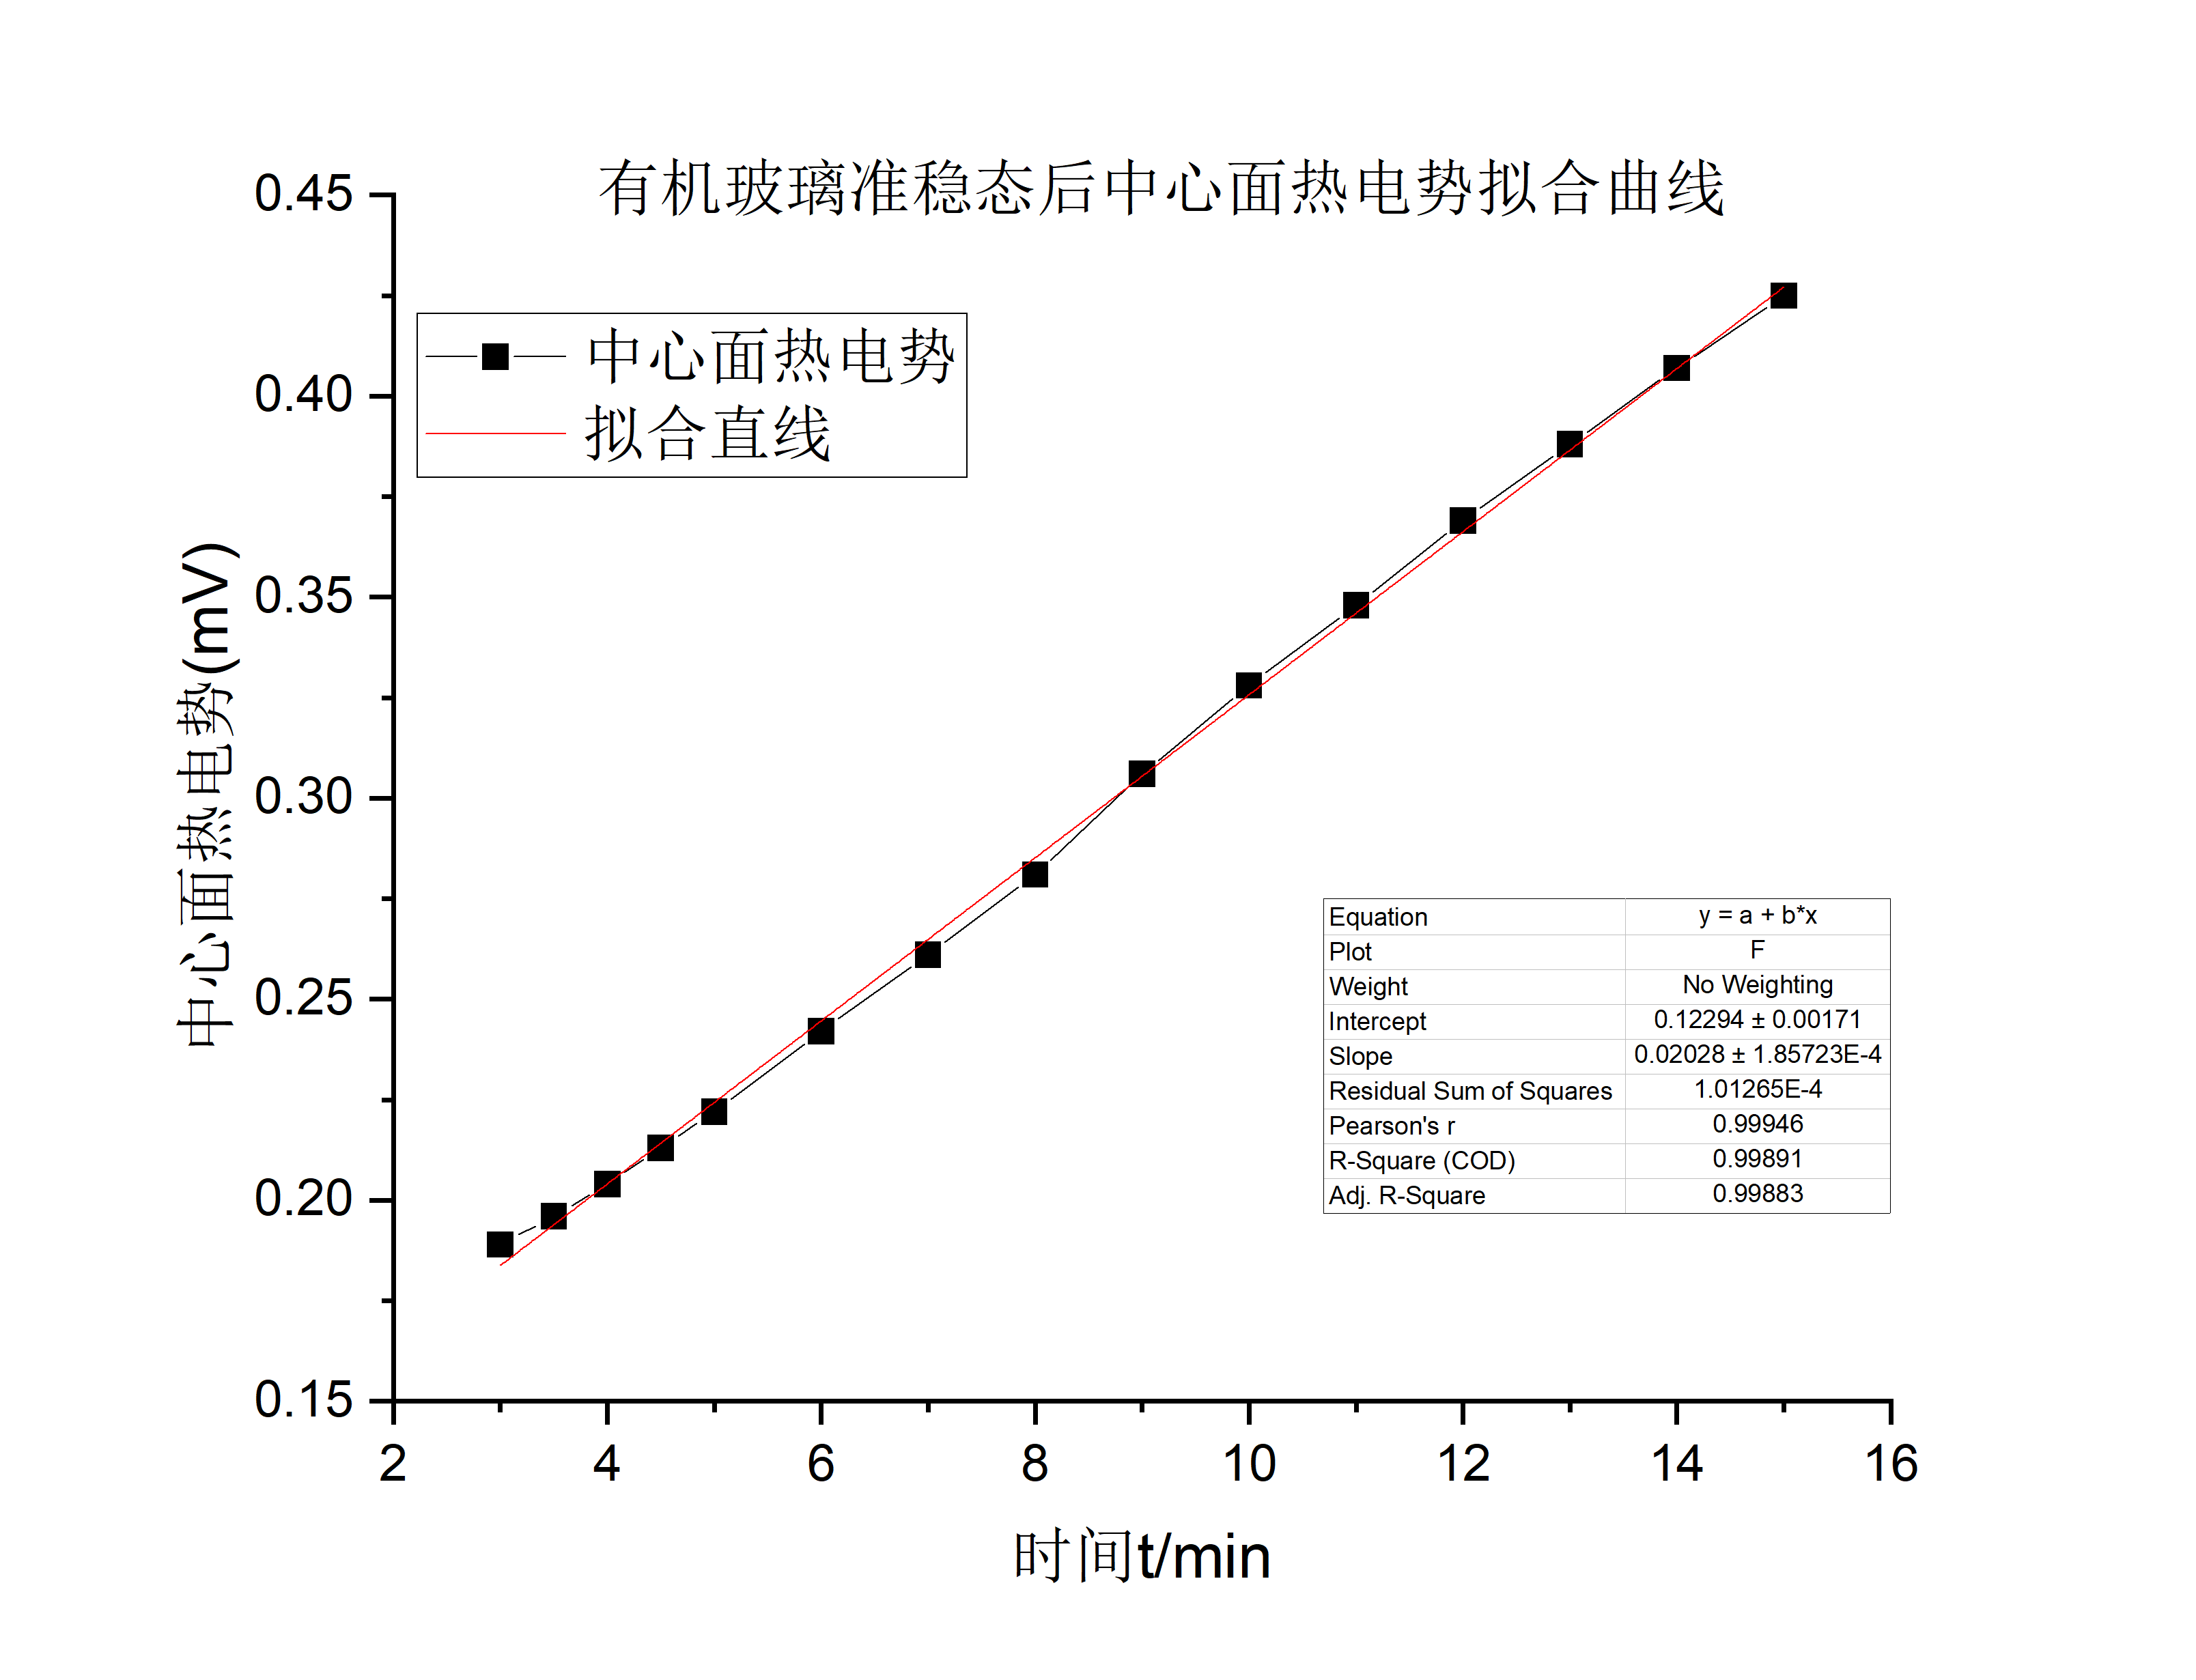
\includegraphics[width=0.4\textwidth]{img//6c.png}
	\label{fig:6c}
	\caption{}
\end{figure}
经准稳态后线性拟合得每分钟温升势电势$\varDelta V=0.02028mV$.
\begin{align*}
	&\frac{dt}{d\tau}=\frac{\varDelta V}{60\times 0.04}=0.00845K/s\\
    &C=\frac{q_c}{\rho_1 R_1 \frac{dt}{d\tau}}=2105.82J/kg\cdot K
\end{align*}

计算得比热$C=2105.82J/kg\cdot K$.


\subsection{测橡胶样品的导热系数和比热容}
\begin{figure}[!h]
	\centering
	\subfloat[]{\label{fig:7a}
	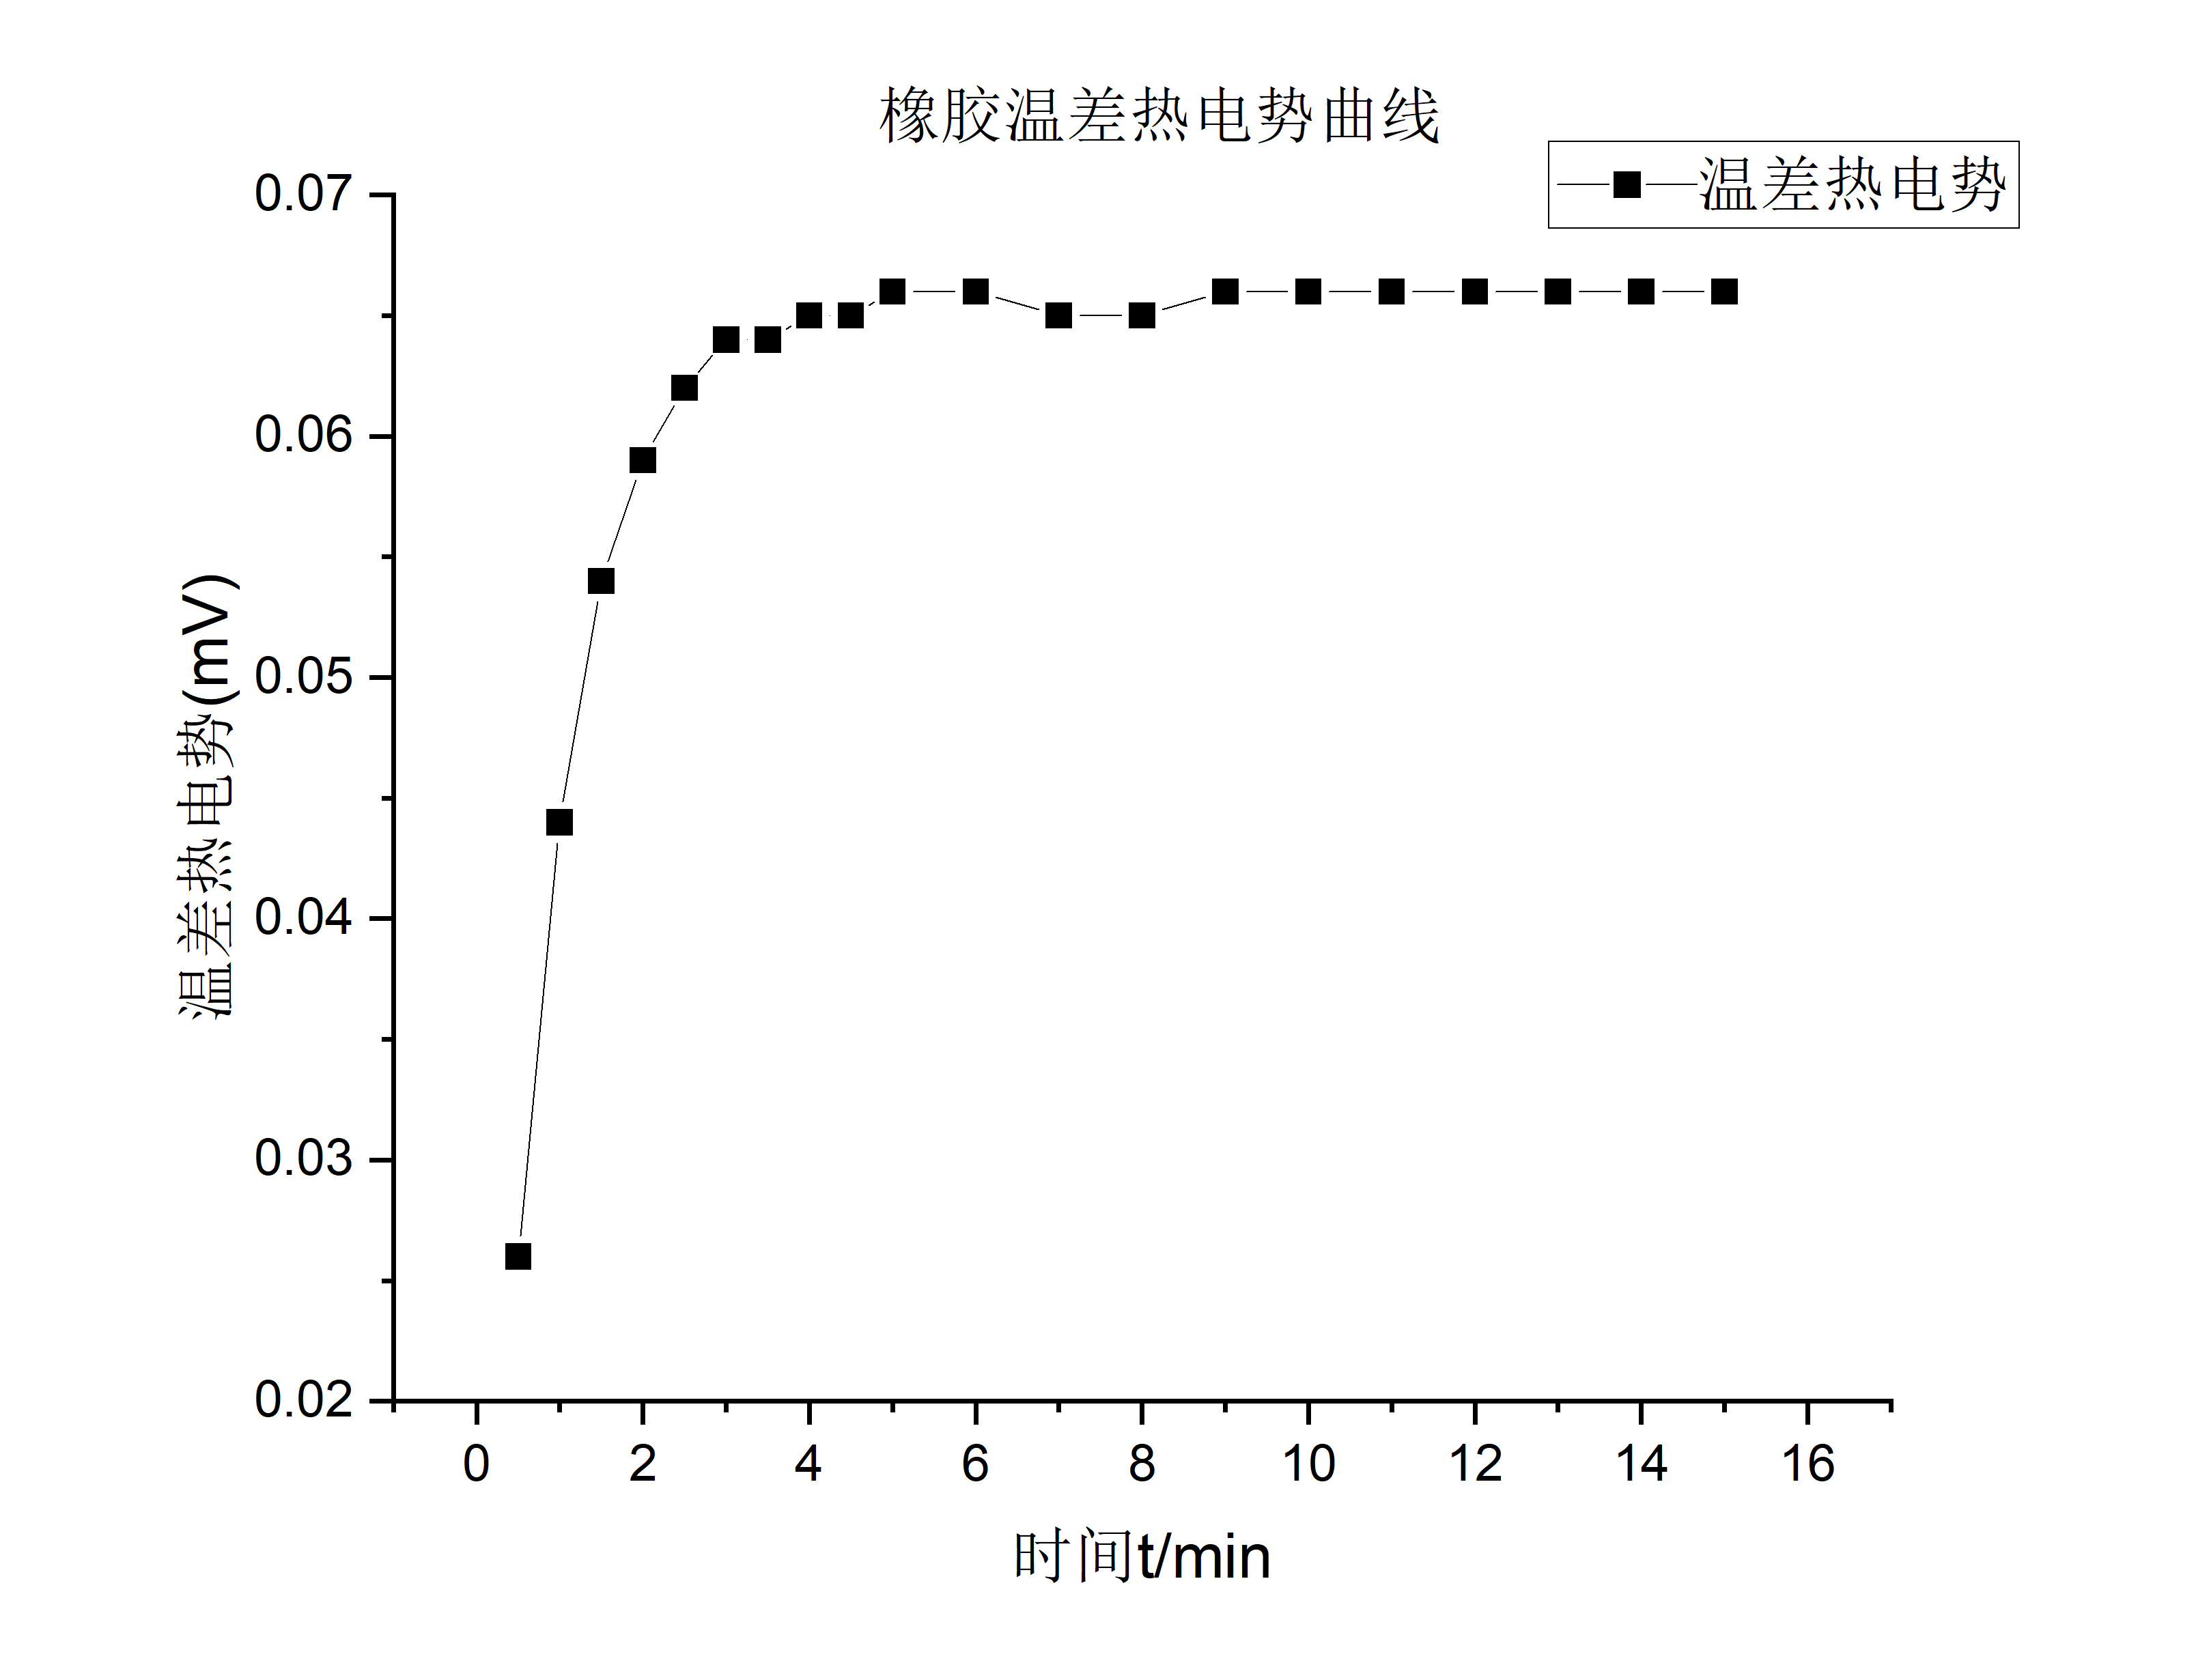
\includegraphics[width=0.23\textwidth]{img//7a.png}
	}	
	\subfloat[]{\label{fig:7b}
	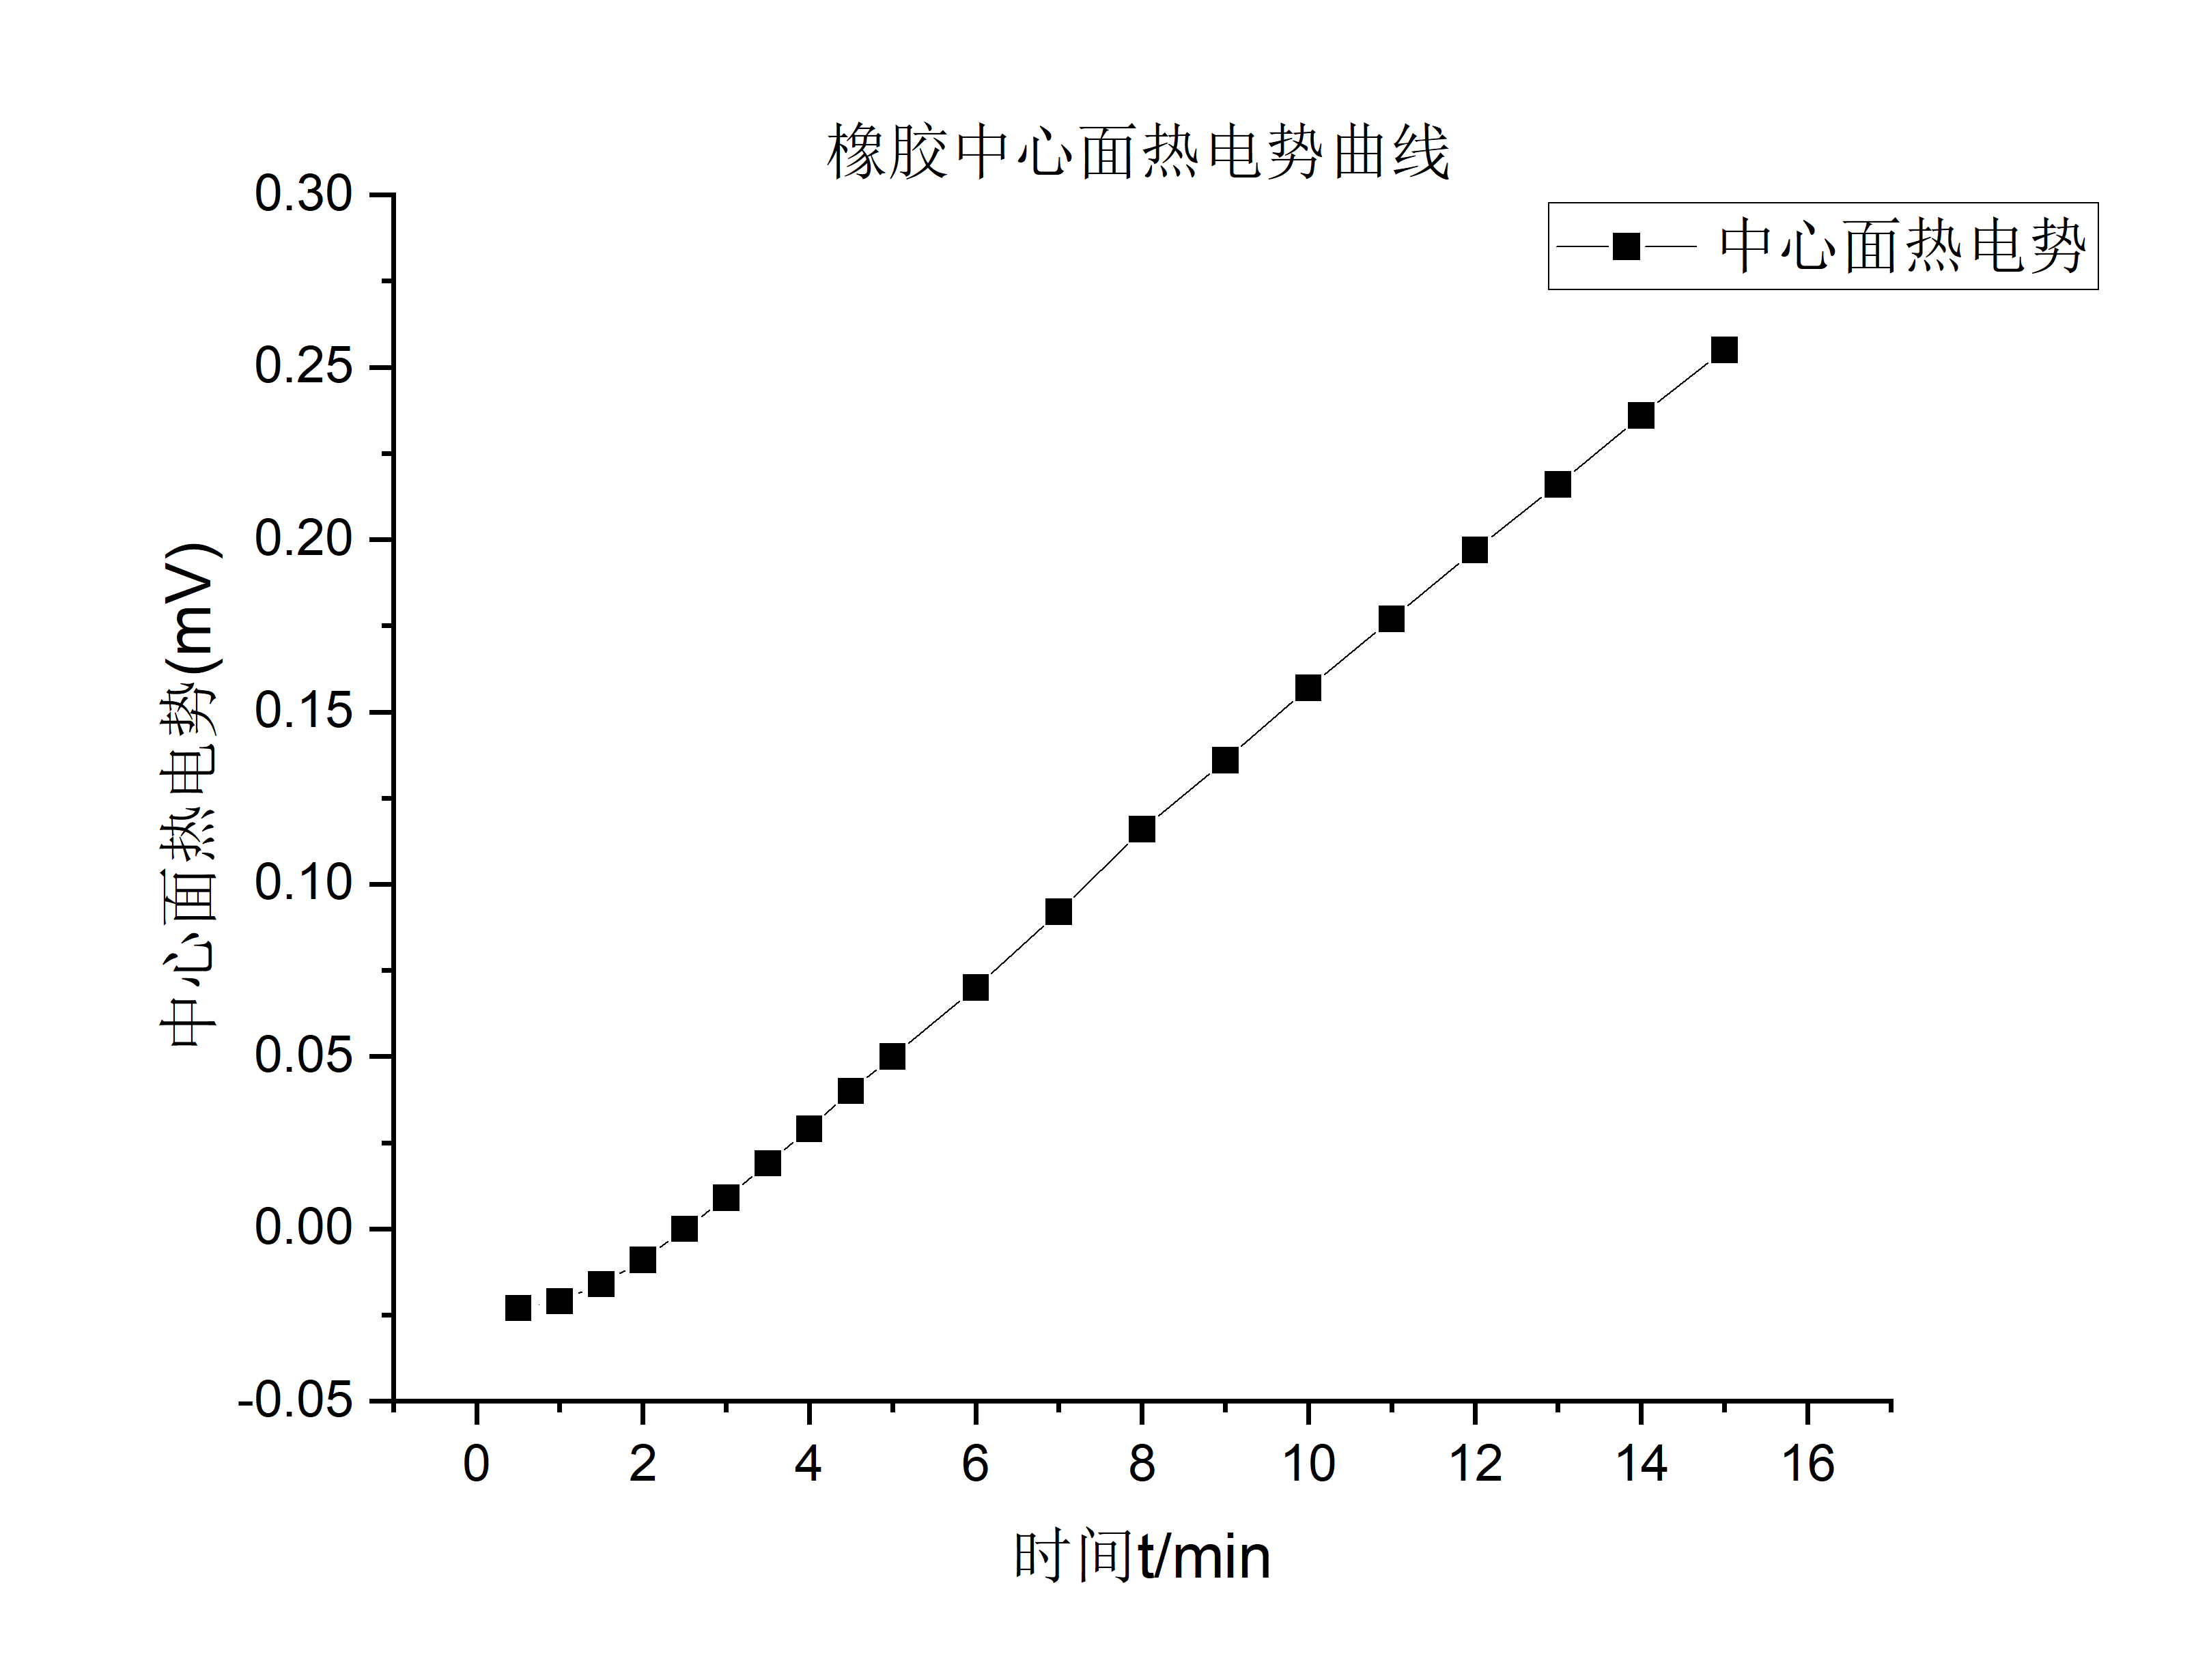
\includegraphics[width=0.23\textwidth]{img//7b.png}
	}
	\caption{橡胶实验数据}
\end{figure}

由实验记录得,在第6分钟处于准稳态。此时温差热电势$V_t=0.066mV$.

\begin{align*}
	&\varDelta t =\frac{V_t}{0.04}=1.655K\\
    &\lambda=\frac{q_c R_2}{2\varDelta t}=0.658W/mK
\end{align*}

计算得热导系数$\lambda=0.658mK$


\begin{figure}[!h]
	\centering
	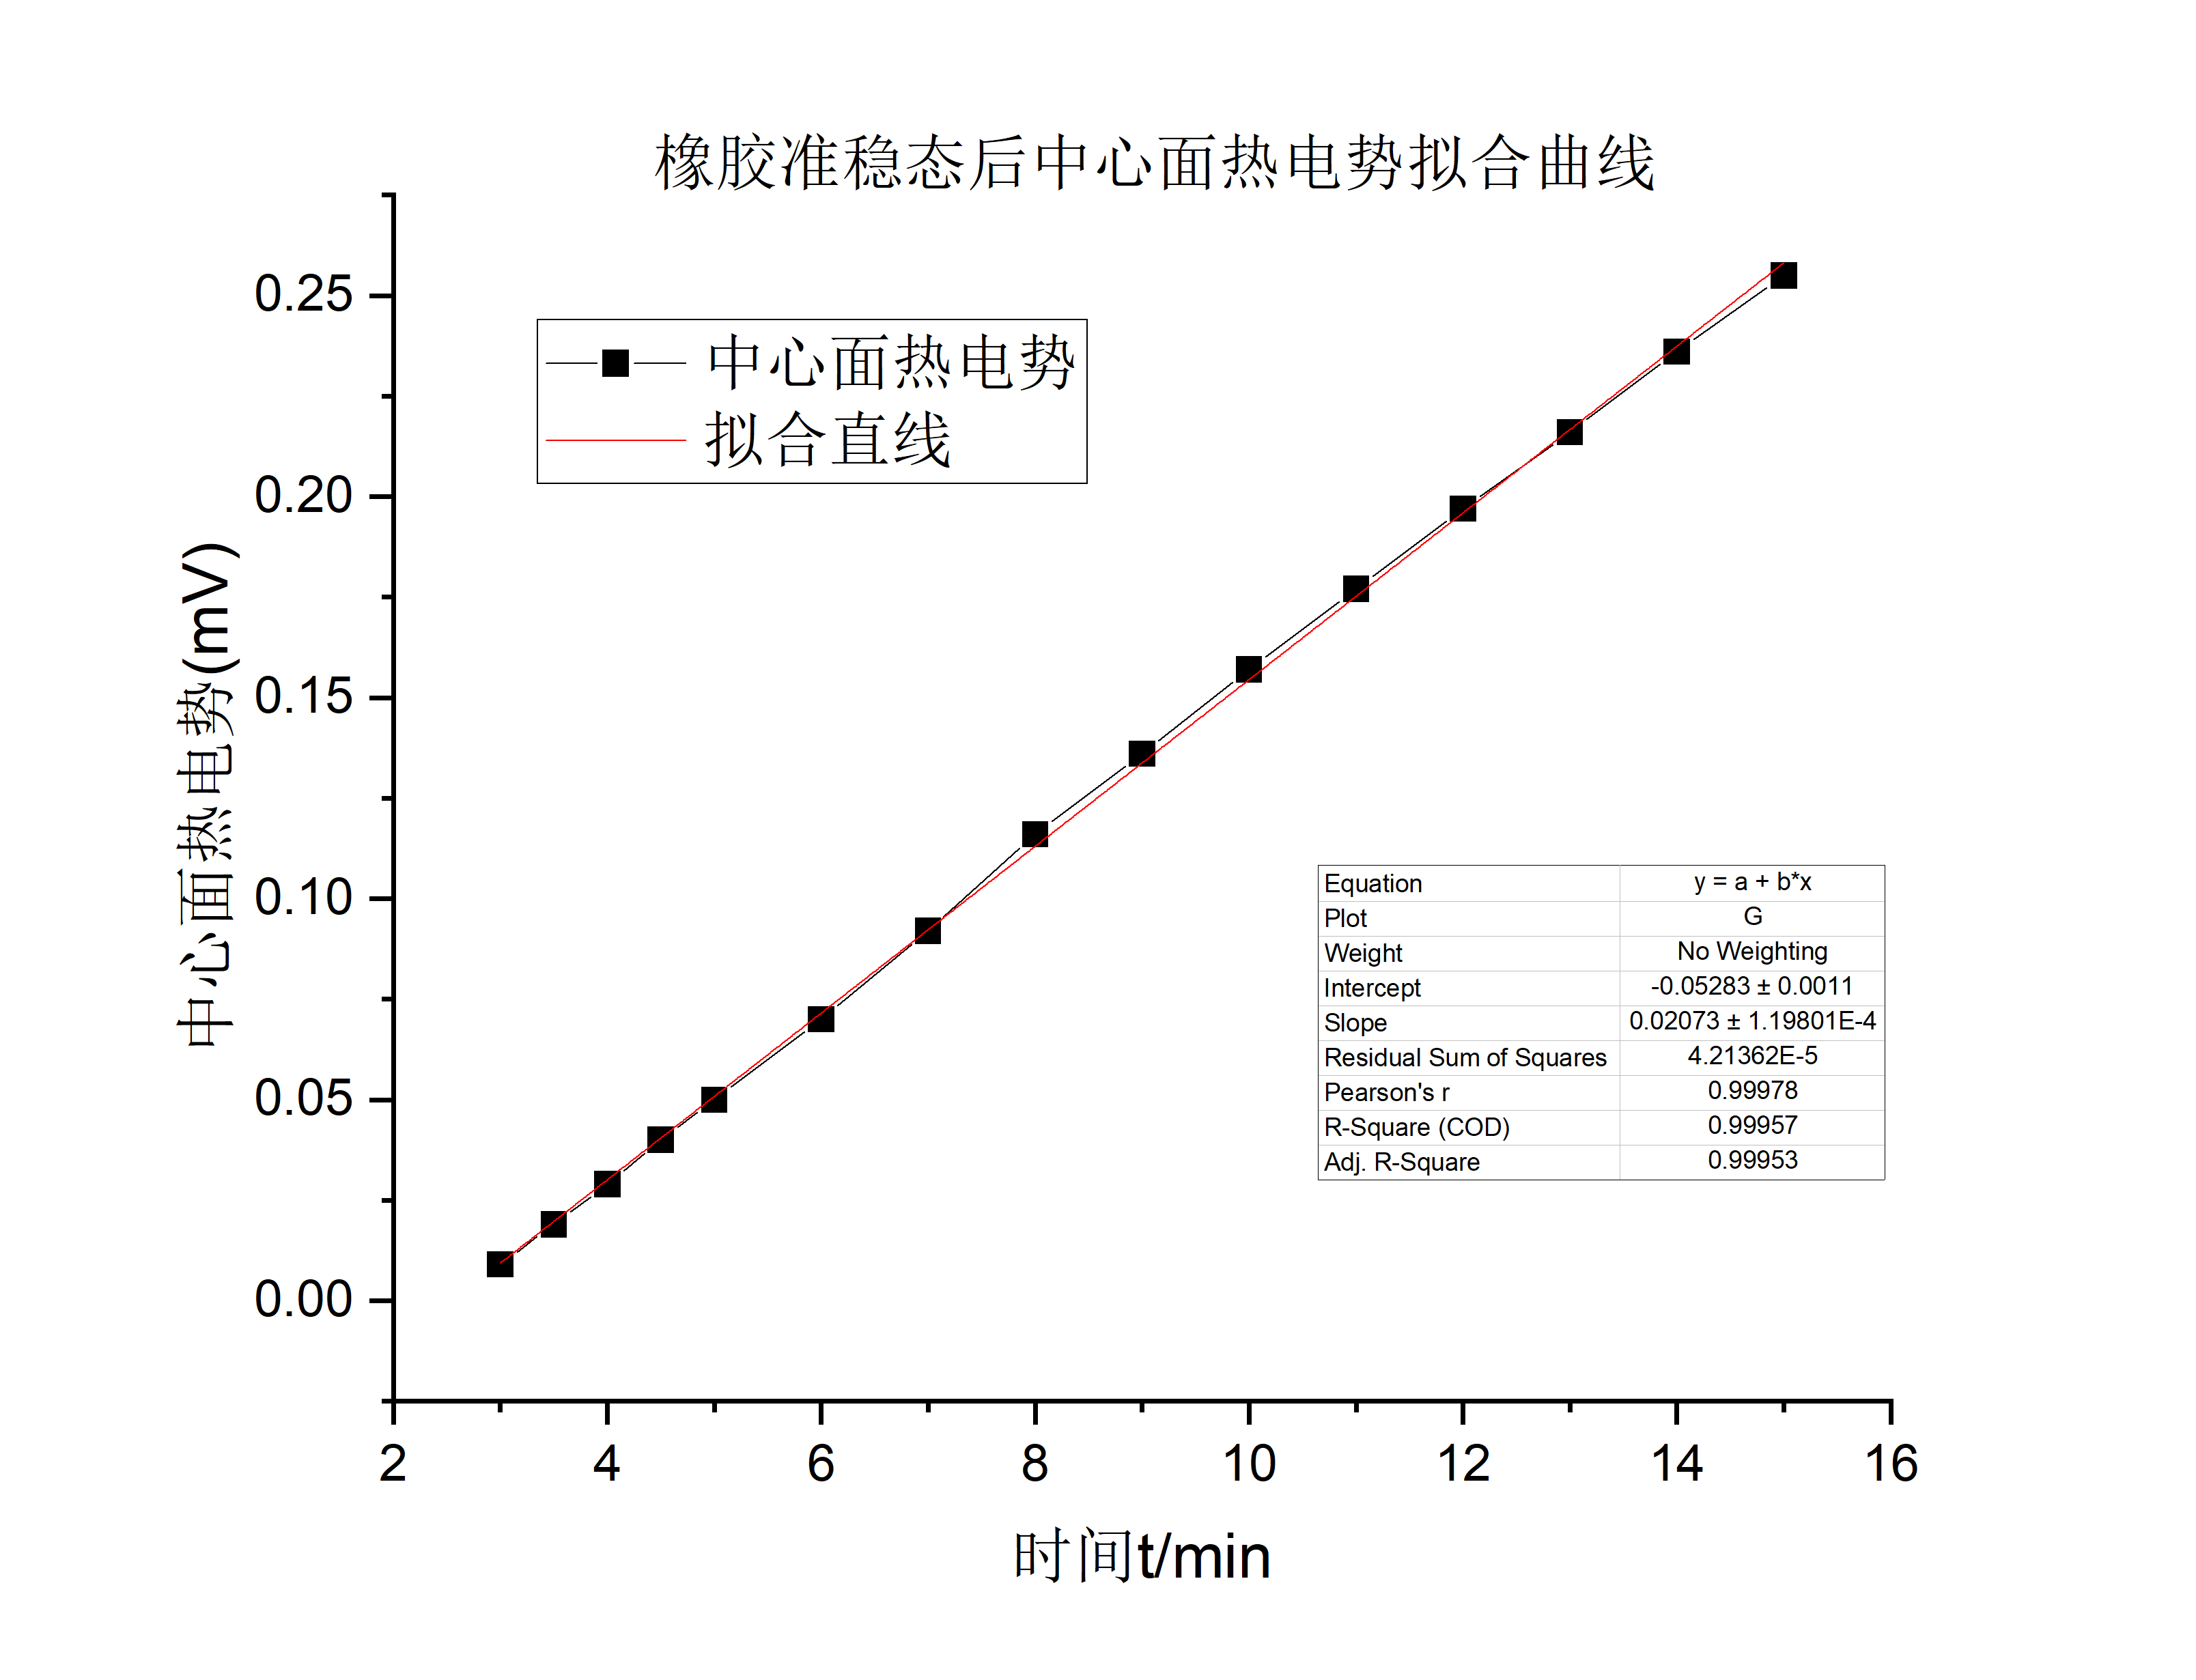
\includegraphics[width=0.4\textwidth]{img//7c.png}
	\label{fig:7c}
	\caption{}
\end{figure}
经准稳态后线性拟合得每分钟温升势电势$\varDelta V=0.02073mV$
\begin{align*}
	&\frac{dt}{d\tau}=\frac{\varDelta V}{60\times 0.04}=0.0086375K/s\\
    &C=\frac{q_c}{\rho_2 R_2 \frac{dt}{d\tau}}=1771.38J/kg\cdot K
\end{align*}

计算得比热$C=1771.38J/kg\cdot K$.


\section{结~~~论}
有机玻璃的导热系数与比热参考值分别为:

$\lambda_0=0.19W/mK$,$C_0=1464/kg\cdot K$

相对误差:
\begin{align*}
	&E_{\lambda}=\left\lvert \frac{\lambda-\lambda_0}{\lambda_0}\right\rvert \times 100\%= 38.9\%\\
    &E_c=\left\lvert \frac{C-C_0}{C_0}\right\rvert \times \%=43.8\%
\end{align*}

橡胶的导热系数与比热参考值分别为:

$\lambda_0=0.426W/mK$,$C_0=1700J/kg\cdot K$

相对误差:
\begin{align*}
	&E_{\lambda}=\left\lvert \frac{\lambda-\lambda_0}{\lambda_0}\right\rvert \times 100\%= 54.5\%\\
    &E_c=\left\lvert \frac{C-C_0}{C_0}\right\rvert \times \%=4.20\%
\end{align*}

均存在误差,造成误差的原因可能是实验非无限大平板,热量并非只在厚度方向传播,
导致热量散失,温差偏小。
此外热电偶由于人为操作(更换被测样品)等原因有损坏,热电常数不严格为0.04mV/K.

综上所述,有机玻璃导热性能不如橡胶;在升高或降低相同温度时,橡胶吸收或放出的热量比有机玻璃多。
\section{参考文献}
\printbibliography[title=参考文献]
[1]沈韩. 基础物理实验[M]. 科学出版社, 2015.

 



%%begin------------------英文摘要------------------------%%

\twocolumn[
\begin{@twocolumnfalse}
	\renewcommand{\abstractname} {} %不显示摘要名字
	\begin{center}%
	    {\LARGE\bfseries Measurement of thermal conductivity of defective conductors (quasi steady state method)\footnotemark[1]  \par}%
	    \vskip 1.4em%
	    {\large
	     \lineskip .75em%
	      \begin{tabular}[t]{c}%
	        \large XXX$^{1}$
	      \end{tabular}\footnotemark[2] \par
	      }%
	      \vskip 0.4em%
	    {\normalsize 1 School of Physics, Sun Yat-sen University, Guangzhou  { \rm 510275}, China}
	\end{center}
	\begin{abstract}
		\vspace{-2em}  %缩小abstract和center(以及maketitle)的间距
	    	{\bf Abstract:}
	     {\small Heat conduction of a thermal conductor follows the heat conduction equation.
		 Thermal conductivity and specific heat are two important parameters to describe thermal conductivity of thermal conductor.
		 In this experiment, we based on thermocouple temperature measurement, using quasi-steady state method to measure the thermal conductivity and specific heat of plexiglass materials. 
		 Then we tried the same on rubber materials in order to explore the thermal conductivity law of bad conductor.
		 Experiment measured organic glass materials for specific heat is $2105.82 J kg^{-1}\ ^{\circ}C^{-1}$, coefficient of thermal conductivity is $\lambda = 0.264 Wm^{-1}K^{-1}$.
		 Rubber material for specific heat is $1771.38 J kg^{-1}\ ^{\circ}C^{-1}$, coefficient of thermal conductivity is $\lambda = 0.658 Wm^{-1}K^{-1} $.}
		 \par% Height of empty new line.}
	  	\par%空的新行的高度。
		\textbf{Key words}:Quasi steady state method, bad conductor, thermocouple, specific heat, thermal conductivity
	\end{abstract}
\end{@twocolumnfalse}
]
\clearpage
	\subsection*{【思考题】}
	\subsubsection*{1.样品导热系数与温度有什么关系?}
	答: 纯金属的导热系数一般随温度升高而降低。除水、甘油外,绝大多数液体导热系数对温度升高而略有减小。气体的导热系数随温度升高而增大。非晶物质随温度升高而增大。

	\subsubsection*{2.样品导热系数的大小与导热性能有什么关系?}
	答: 导热系数越大,导热性能越优良。
	\subsubsection*{3.分析实验主要误差来源。}
\begin{enumerate}
	\item 温度测量时的误差,影响所用的热电偶温度传感器的传导效率,以及由于热电偶输出电压是非线性关系,影响热电偶转化为温度的准确性。
	\item 确定热流密度$q_c$的误差。因为无法直接测量热流密度,用加热功率密度的一半代替。热量耗散、加热器功率不稳定或分布不均匀、两侧样品不完全相同导致热阻不同等因素影响热流密度的准确性。
	\item 试件的实际尺寸与代入值不同产生的误差。
	\item 计算假定初始温度分布均匀,实际情况无法推测。
\end{enumerate}
    
\subsubsection*{4.本实验中如何实现稳定导热?如何判定已经到达稳定导热状态?}
答:实验使用的超薄型加热器,使得加热功率在加热面上均匀并可精准控制。在加热器两侧放置相同样品,保证热阻相同。
用热电偶传感器准确测量加热面和中心面热电势,精准反应温度变化。当温差热电势和每分钟温升热电势趋于稳定值,或在误差范围内作微小波动,
则可判定达到稳定导热状态。

\footnotetext[1]{{Supported and taught by Luyoutang, School of Physics, Sun Yat-sen University}}
\footnotetext[2]{{Corresponding author. E-mail:\url{xxxx@mail2.sysu.edu.cn}}}
%%end--------------------英文摘要------------------------%%


\end{document}
